% Options for packages loaded elsewhere
\PassOptionsToPackage{unicode}{hyperref}
\PassOptionsToPackage{hyphens}{url}
%
\documentclass[
  17pt,
  letterpaper,
  ignorenonframetext,
  aspectratio=169,
  handout]{beamer}
\usepackage{pgfpages}
\setbeamertemplate{caption}[numbered]
\setbeamertemplate{caption label separator}{: }
\setbeamercolor{caption name}{fg=normal text.fg}
\beamertemplatenavigationsymbolsempty
% Prevent slide breaks in the middle of a paragraph
\widowpenalties 1 10000
\raggedbottom
\setbeamertemplate{part page}{
  \centering
  \begin{beamercolorbox}[sep=16pt,center]{part title}
    \usebeamerfont{part title}\insertpart\par
  \end{beamercolorbox}
}
\setbeamertemplate{section page}{
  \centering
  \begin{beamercolorbox}[sep=12pt,center]{part title}
    \usebeamerfont{section title}\insertsection\par
  \end{beamercolorbox}
}
\setbeamertemplate{subsection page}{
  \centering
  \begin{beamercolorbox}[sep=8pt,center]{part title}
    \usebeamerfont{subsection title}\insertsubsection\par
  \end{beamercolorbox}
}
\AtBeginPart{
  \frame{\partpage}
}
\AtBeginSection{
  \ifbibliography
  \else
    \frame{\sectionpage}
  \fi
}
\AtBeginSubsection{
  \frame{\subsectionpage}
}

\usepackage{amsmath,amssymb}
\usepackage{lmodern}
\usepackage{iftex}
\ifPDFTeX
  \usepackage[T1]{fontenc}
  \usepackage[utf8]{inputenc}
  \usepackage{textcomp} % provide euro and other symbols
\else % if luatex or xetex
  \usepackage{unicode-math}
  \defaultfontfeatures{Scale=MatchLowercase}
  \defaultfontfeatures[\rmfamily]{Ligatures=TeX,Scale=1}
  \setmainfont[BoldFont = SF Pro Text Semibold, Scale =
MatchLowercase]{SF Pro Text Light}
\fi
\usecolortheme{wolverine}
\usefonttheme{serif} % use mainfont rather than sansfont for slide text
\useinnertheme{default}
\useoutertheme{miniframes}
% Use upquote if available, for straight quotes in verbatim environments
\IfFileExists{upquote.sty}{\usepackage{upquote}}{}
\IfFileExists{microtype.sty}{% use microtype if available
  \usepackage[]{microtype}
  \UseMicrotypeSet[protrusion]{basicmath} % disable protrusion for tt fonts
}{}
\makeatletter
\@ifundefined{KOMAClassName}{% if non-KOMA class
  \IfFileExists{parskip.sty}{%
    \usepackage{parskip}
  }{% else
    \setlength{\parindent}{0pt}
    \setlength{\parskip}{6pt plus 2pt minus 1pt}}
}{% if KOMA class
  \KOMAoptions{parskip=half}}
\makeatother
\usepackage{xcolor}
\newif\ifbibliography
\setlength{\emergencystretch}{3em} % prevent overfull lines
\setcounter{secnumdepth}{-\maxdimen} % remove section numbering


\providecommand{\tightlist}{%
  \setlength{\itemsep}{0pt}\setlength{\parskip}{0pt}}\usepackage{longtable,booktabs,array}
\usepackage{calc} % for calculating minipage widths
\usepackage{caption}
% Make caption package work with longtable
\makeatletter
\def\fnum@table{\tablename~\thetable}
\makeatother
\usepackage{graphicx}
\makeatletter
\def\maxwidth{\ifdim\Gin@nat@width>\linewidth\linewidth\else\Gin@nat@width\fi}
\def\maxheight{\ifdim\Gin@nat@height>\textheight\textheight\else\Gin@nat@height\fi}
\makeatother
% Scale images if necessary, so that they will not overflow the page
% margins by default, and it is still possible to overwrite the defaults
% using explicit options in \includegraphics[width, height, ...]{}
\setkeys{Gin}{width=\maxwidth,height=\maxheight,keepaspectratio}
% Set default figure placement to htbp
\makeatletter
\def\fps@figure{htbp}
\makeatother

\captionsetup[figure]{labelformat=empty}
\usepackage{pgfpages}
\setbeamertemplate{itemize item}[circle]
\setbeamertemplate{footline}[frame number]{}
\mode<handout>{\pgfpagesuselayout{6 on 1}[letterpaper, border shrink=8mm]}
\AtBeginSection{%
   \begin{frame}
       \tableofcontents[currentsection]
   \end{frame}
}
\makeatletter
\makeatother
\makeatletter
\makeatother
\makeatletter
\@ifpackageloaded{caption}{}{\usepackage{caption}}
\AtBeginDocument{%
\ifdefined\contentsname
  \renewcommand*\contentsname{Table of contents}
\else
  \newcommand\contentsname{Table of contents}
\fi
\ifdefined\listfigurename
  \renewcommand*\listfigurename{List of Figures}
\else
  \newcommand\listfigurename{List of Figures}
\fi
\ifdefined\listtablename
  \renewcommand*\listtablename{List of Tables}
\else
  \newcommand\listtablename{List of Tables}
\fi
\ifdefined\figurename
  \renewcommand*\figurename{Figure}
\else
  \newcommand\figurename{Figure}
\fi
\ifdefined\tablename
  \renewcommand*\tablename{Table}
\else
  \newcommand\tablename{Table}
\fi
}
\@ifpackageloaded{float}{}{\usepackage{float}}
\floatstyle{ruled}
\@ifundefined{c@chapter}{\newfloat{codelisting}{h}{lop}}{\newfloat{codelisting}{h}{lop}[chapter]}
\floatname{codelisting}{Listing}
\newcommand*\listoflistings{\listof{codelisting}{List of Listings}}
\makeatother
\makeatletter
\@ifpackageloaded{caption}{}{\usepackage{caption}}
\@ifpackageloaded{subcaption}{}{\usepackage{subcaption}}
\makeatother
\makeatletter
\@ifpackageloaded{tcolorbox}{}{\usepackage[many]{tcolorbox}}
\makeatother
\makeatletter
\@ifundefined{shadecolor}{\definecolor{shadecolor}{rgb}{.97, .97, .97}}
\makeatother
\makeatletter
\makeatother
\ifLuaTeX
  \usepackage{selnolig}  % disable illegal ligatures
\fi
\IfFileExists{bookmark.sty}{\usepackage{bookmark}}{\usepackage{hyperref}}
\IfFileExists{xurl.sty}{\usepackage{xurl}}{} % add URL line breaks if available
\urlstyle{same} % disable monospaced font for URLs
\hypersetup{
  pdftitle={Knowledge and Reality, Lecture 05},
  pdfauthor={Brian Weatherson},
  hidelinks,
  pdfcreator={LaTeX via pandoc}}

\title{Knowledge and Reality, Lecture 05}
\author{Brian Weatherson}
\date{2022-09-14}

\begin{document}
\frame{\titlepage}
\ifdefined\Shaded\renewenvironment{Shaded}{\begin{tcolorbox}[interior hidden, frame hidden, borderline west={3pt}{0pt}{shadecolor}, boxrule=0pt, sharp corners, enhanced, breakable]}{\end{tcolorbox}}\fi

\hypertarget{review-and-finishing-up}{%
\section{Review (And Finishing Up)}\label{review-and-finishing-up}}

\begin{frame}{Testimony}
\protect\hypertarget{testimony}{}
\begin{itemize}[<+->]
\tightlist
\item
  We spent the last two classes on testimony, and in particular on when
  it is rational to believe something on the basis of testimony.
\end{itemize}
\end{frame}

\begin{frame}{Two Theories}
\protect\hypertarget{two-theories}{}
\begin{itemize}[<+->]
\tightlist
\item
  Testimony is basic, and rationally believing testimony requires just
  an absence of reasons for doubt.
\item
  Testimonial belief is inferential, and rationally believing testimony
  requires reason to think the speaker is telling the truth.
\end{itemize}
\end{frame}

\begin{frame}{Two Theories}
\protect\hypertarget{two-theories-1}{}
\begin{description}[<+->]
\tightlist
\item[Reductionism]
Rationally believing testimony requires reasons to accept.
\item[Anti-Reductionism]
Rationally believing testimony requires absence of reasons to reject.
\end{description}

These come apart when there are no reasons to accept or reject.
\end{frame}

\begin{frame}{Philosophy and Psychology}
\protect\hypertarget{philosophy-and-psychology}{}
General background assumption:

\begin{itemize}[<+->]
\tightlist
\item
  People are rational.
\item
  So which of the theories of rationality is correct is linked to
  empirical work on what people actually do.
\end{itemize}
\end{frame}

\begin{frame}{Over-Intellectualisation}
\protect\hypertarget{over-intellectualisation}{}
Anti-reductionists think that reductionists
\textbf{over-intellectualise} testimony reception.

\begin{itemize}[<+->]
\tightlist
\item
  They say their opponents add mental steps to what's a much simpler
  process.
\item
  This was a common late C20 response to philosophical views in many
  topics.
\end{itemize}
\end{frame}

\begin{frame}{Paris School}
\protect\hypertarget{paris-school}{}
\begin{itemize}[<+->]
\tightlist
\item
  A general response to over-intellectualisation objections in many
  domains.
\end{itemize}
\end{frame}

\begin{frame}{Paris School}
\protect\hypertarget{paris-school-1}{}
People do have lots of rules, life hacks in 2010s lingo, to get around.
But\ldots{}

\begin{itemize}[<+->]
\tightlist
\item
  They don't apply them in high stakes cases.
\item
  And they don't apply them when it is obvious they would fail.
\item
  So they must be checking every time whether this is a
  high-stakes/obvious-fail situation.
\end{itemize}
\end{frame}

\begin{frame}{Vigilance}
\protect\hypertarget{vigilance}{}
My favorite example: walking down a busy street or corridor.

\begin{itemize}[<+->]
\tightlist
\item
  We somehow track everyone, while attending to almost no one.
\item
  Really big question: How on earth do we do this, and can we invent a
  machine that does something similar?
\end{itemize}
\end{frame}

\begin{frame}{Vigilant Hearers}
\protect\hypertarget{vigilant-hearers}{}
Sperber et al think that we are also vigilant in hearing.

\begin{itemize}[<+->]
\tightlist
\item
  Everything gets a rough check, almost always subconsciously.
\item
  Some things get more thorough check.
\end{itemize}
\end{frame}

\begin{frame}{Red Flags}
\protect\hypertarget{red-flags}{}
\begin{itemize}[<+->]
\tightlist
\item
  New informants
\item
  Surprising that info is either true or known
\item
  Reason to deceive
\item
  High stakes
\end{itemize}
\end{frame}

\begin{frame}{Big Question}
\protect\hypertarget{big-question}{}
Is this plausible as a model of how human hearers operate?
\end{frame}

\begin{frame}{Today}
\protect\hypertarget{today}{}
\begin{itemize}[<+->]
\tightlist
\item
  What kind of thing is rationality?
\end{itemize}
\end{frame}

\begin{frame}{Terminology}
\protect\hypertarget{terminology}{}
\begin{itemize}[<+->]
\tightlist
\item
  The writers we'll look at move back and forth between talking about
  \textbf{rational} belief and \textbf{justified} belief.
\item
  I'm not going to get into whether these are different, or what the
  differences might be.
\item
  Treat them as the same, knowing that, as always, it might be more
  complicated than that.
\end{itemize}
\end{frame}

\hypertarget{internalism-and-externalism}{%
\section{Internalism and
Externalism}\label{internalism-and-externalism}}

\begin{frame}{What Does Rationality Depend on?}
\protect\hypertarget{what-does-rationality-depend-on}{}
Imagine that one person is rational, and another irrational.

\begin{itemize}[<+->]
\tightlist
\item
  How must they differ?
\item
  Could they be internally alike?
\end{itemize}
\end{frame}

\begin{frame}{Internalism}
\protect\hypertarget{internalism}{}
Rationality is a function of what's internal to the person.

\begin{itemize}[<+->]
\tightlist
\item
  Two people who are internally alike are either both rational, or both
  irrational.
\end{itemize}
\end{frame}

\begin{frame}{Internal?}
\protect\hypertarget{internal}{}
What does `internal' mean here? Two prominent options (which I'm stating
but won't go into)

\begin{enumerate}[<+->]
\tightlist
\item
  Physical, e.g., brain states, sense organs, etc.
\item
  Phenomenological, e.g., feelings, sensations, etc. This is sometimes
  called \textbf{access internalism}; rationality just depends on what
  the thinker has access to.
\end{enumerate}
\end{frame}

\begin{frame}{How Does It Depend?}
\protect\hypertarget{how-does-it-depend}{}
Again, two big theories, though these aren't exclusive or exhaustive.

\begin{enumerate}[<+->]
\tightlist
\item
  Evidential; rationality is a matter of having beliefs based in the
  right way in evidence, which (on this view) is a special kind of
  internal state. Sometimes this is called foundationalism.
\item
  Coherence; rationality is a matter of internal states cohering.
\end{enumerate}
\end{frame}

\begin{frame}{How Does It Depend?}
\protect\hypertarget{how-does-it-depend-1}{}
We'll come back to this, because some of the objections to internalism
target just one or the other theory.
\end{frame}

\begin{frame}{Externalism}
\protect\hypertarget{externalism}{}
Externalism is simply the denial of internalism.

\begin{itemize}[<+->]
\tightlist
\item
  It says that sometimes internal duplicates differ in rationality.
\end{itemize}
\end{frame}

\begin{frame}{Strong Externalism}
\protect\hypertarget{strong-externalism}{}
A really strong form of externalism says that only external factors
matter to rationality.

\begin{itemize}[<+->]
\tightlist
\item
  This is not a popular view, though the Srinivasan paper we'll read
  next comes very close to defending it.
\item
  But external here typically means ``not exclusively internal''.
\end{itemize}
\end{frame}

\begin{frame}{Process Reliabilism}
\protect\hypertarget{process-reliabilism}{}
The most popular form of externalism these days is \textbf{process
reliabilism}. This has two parts.

\begin{itemize}[<+->]
\tightlist
\item
  In general, rational beliefs are those that are produced by reliable
  processes.
\item
  But there is an exception; beliefs that fail some internalist test
  might be `defeated', and not rational.
\end{itemize}
\end{frame}

\begin{frame}{Process Reliabilism}
\protect\hypertarget{process-reliabilism-1}{}
Process reliabilism is most associated with Alvin Goldman, a former
professor here at UM.

\begin{itemize}[<+->]
\tightlist
\item
  Indeed, I think some of the most important statements of it were from
  his time at UM.
\item
  Another important figure (who we'll read in a related context soon) is
  the Cuban-American philosopher Ernest Sosa.
\end{itemize}
\end{frame}

\hypertarget{why-internalism}{%
\section{Why Internalism}\label{why-internalism}}

\begin{frame}{Three Reasons}
\protect\hypertarget{three-reasons}{}
This is an enormous debate, but I'll pull out three reasons that I think
are significant.

\begin{enumerate}[<+->]
\tightlist
\item
  Anti-luck.
\item
  Cases.
\item
  Evil Demons
\end{enumerate}
\end{frame}

\begin{frame}{Anti-Luck}
\protect\hypertarget{anti-luck}{}
\begin{itemize}[<+->]
\tightlist
\item
  Saying something is rational is a way of saying that it's not a lucky
  guess, and if it's false, it's unlucky.
\item
  External factors are basically matters of luck.
\item
  So rationality should depend only on internal factors.
\end{itemize}
\end{frame}

\begin{frame}{Cases}
\protect\hypertarget{cases}{}
Lawrence BonJour introduced the following kind of case.

\begin{itemize}[<+->]
\tightlist
\item
  A person has (somehow) acquired clairvoyant powers.
\item
  They have these beliefs about distant parts of the world that just
  come to them.
\item
  And these beliefs are true.
\end{itemize}
\end{frame}

\begin{frame}{Question}
\protect\hypertarget{question}{}
\begin{enumerate}[<+->]
\tightlist
\item
  Is simply trusting this new clairvoyant sense rational for the person?
\item
  If not, is this a problem for reliabilists.
\end{enumerate}
\end{frame}

\begin{frame}{Evil Demon}
\protect\hypertarget{evil-demon}{}
The evil demon usually comes into epistemology as part of an argument
about scepticism.

\begin{itemize}[<+->]
\tightlist
\item
  E.g., you don't know you're not being deceived by an evil demon, so
  you don't know that you have hands.
\item
  But here is gets used for a debate about rationality.
\end{itemize}
\end{frame}

\begin{frame}{Sympathy for the Devil (Victim)}
\protect\hypertarget{sympathy-for-the-devil-victim}{}
Imagine a person who seems, from the inside, to be just like an actually
rational person.

\begin{itemize}[<+->]
\tightlist
\item
  But in fact they are the victim of an evil demon, so their beliefs are
  all false.
\item
  Reliabilists say they are irrational, but they are intuitively
  rational.
\end{itemize}
\end{frame}

\begin{frame}{Question}
\protect\hypertarget{question-1}{}
What should reliabilists say about this case?
\end{frame}

\begin{frame}{Variant}
\protect\hypertarget{variant}{}
Imagine two evil demon victims.

\begin{itemize}[<+->]
\tightlist
\item
  A is, from the inside, a paradigm of rationality.
\item
  B is, from the inside, a conspiracy theorist who leaps to conclusions,
  believes everything he's told, etc., etc.
\end{itemize}
\end{frame}

\begin{frame}{Question}
\protect\hypertarget{question-2}{}
Can reliabilists say something about the intuitive differences between A
and B?
\end{frame}

\hypertarget{why-externalism}{%
\section{Why Externalism}\label{why-externalism}}

\begin{frame}{Three Arguments}
\protect\hypertarget{three-arguments}{}
Again, there are many, but I'll just look at these three.

\begin{enumerate}[<+->]
\tightlist
\item
  Speckled hen
\item
  Why care about rationality?
\item
  Involuntarism
\end{enumerate}
\end{frame}

\begin{frame}{Speckled Hen}
\protect\hypertarget{speckled-hen}{}
\begin{figure}

{\centering 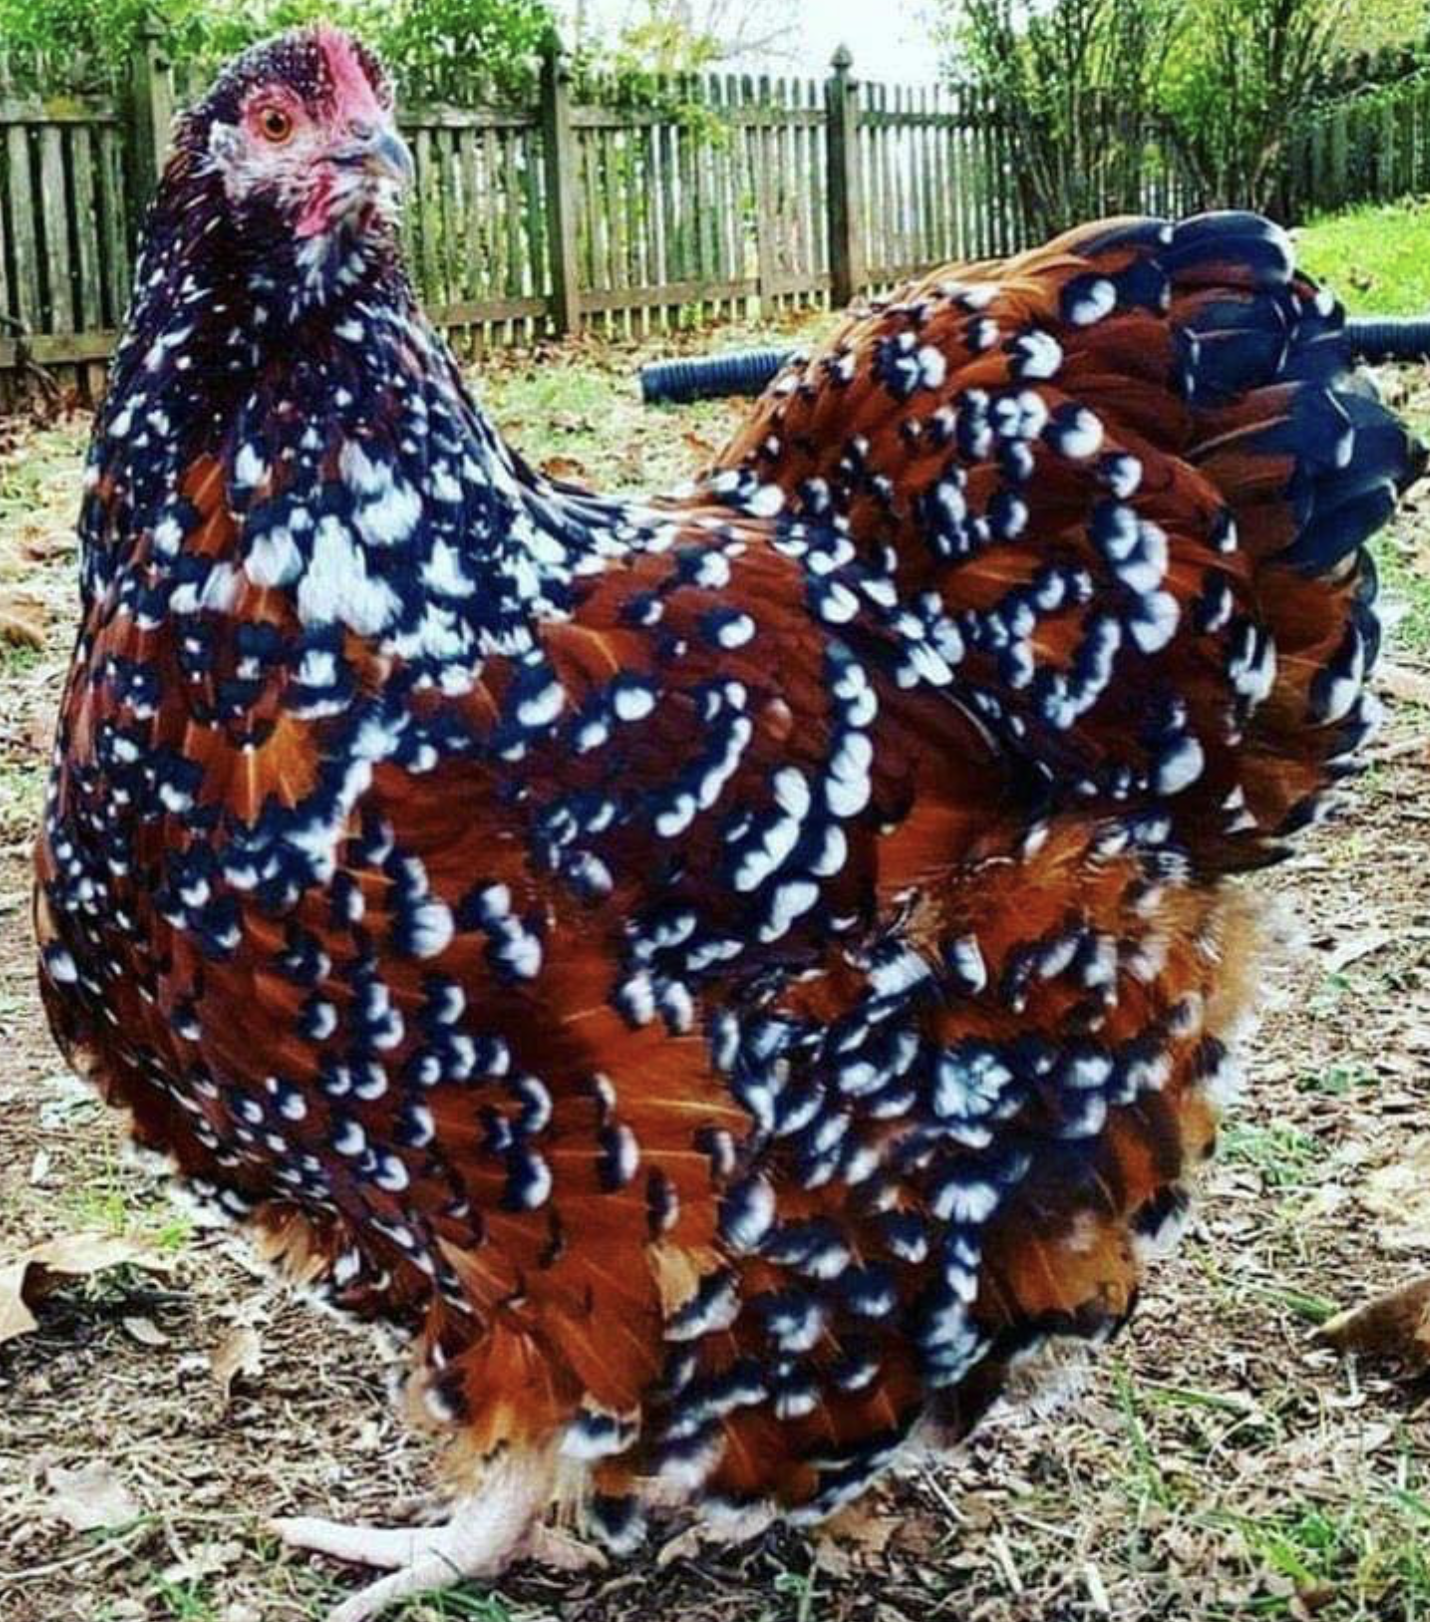
\includegraphics[width=\textwidth,height=0.6\textheight]{../images/hen.jpg}

}

\caption{How many visible white speckles?}

\end{figure}
\end{frame}

\begin{frame}{Speckled Hen}
\protect\hypertarget{speckled-hen-1}{}
\begin{itemize}[<+->]
\tightlist
\item
  The right answer does just depend on your internal states.
\item
  But it seems that any number you came up with by just guessing would
  not be a rational belief.
\item
  So rationality requires more than internal states, it requires a
  reliable connection to the world.
\end{itemize}
\end{frame}

\begin{frame}{Why Care?}
\protect\hypertarget{why-care}{}
Rationality should be something we care about.

\begin{itemize}[<+->]
\tightlist
\item
  But if given a choice between being evidence-responsive, and being
  reliable, we should choose being reliable.
\item
  And same for coherent versus reliable.
\end{itemize}
\end{frame}

\begin{frame}{Why Care?}
\protect\hypertarget{why-care-1}{}
\begin{itemize}[<+->]
\tightlist
\item
  Belief, in some sense, aims at the truth.
\item
  Rationality means something like doing well in believing.
\item
  So, being rational should mean something like doing well in getting to
  the truth.
\item
  That means reliability.
\end{itemize}
\end{frame}

\begin{frame}{Why Care?}
\protect\hypertarget{why-care-2}{}
Are there hand-wavy moves on the previous slide that might not hold up
to strict scrutiny? Yes!
\end{frame}

\begin{frame}{Voluntarism}
\protect\hypertarget{voluntarism}{}
\begin{itemize}[<+->]
\tightlist
\item
  We evaluate the voluntary parts of human behavior by whether they make
  sense, and the involuntary parts by whether they work.
\item
  Belief is involuntary.
\item
  So we should evaluate it by how well it works.
\end{itemize}
\end{frame}

\begin{frame}{Somewhat Concessive}
\protect\hypertarget{somewhat-concessive}{}
\begin{itemize}[<+->]
\tightlist
\item
  This argument concedes that if belief were voluntary, internalism
  would be plausible/correct.
\item
  But, it says, belief is involuntary.
\end{itemize}
\end{frame}

\begin{frame}{Evaluation}
\protect\hypertarget{evaluation}{}
Whether someone has, say, a good or bad digestive system is not a
strictly internal matter.

\begin{itemize}[<+->]
\tightlist
\item
  Having a good digestive system just is being good at digesting common
  foods.
\item
  And what the common foods are is external.
\item
  The involunarists say belief is the same.
\end{itemize}
\end{frame}

\begin{frame}{Two Objections}
\protect\hypertarget{two-objections}{}
\begin{enumerate}[<+->]
\tightlist
\item
  Belief really is voluntary.
\item
  Enough things connected to belief are voluntary that we can use
  something like internalist criteria.
\end{enumerate}
\end{frame}

\begin{frame}{For Next Time}
\protect\hypertarget{for-next-time}{}
We'll look at a very recent contribution to this debate, Amia
Srinivasan's argument for externalism from cases involving oppression.
\end{frame}



\end{document}
